\documentclass[algebra]{subfiles}

\begin{document}
    \section{Характеристический многочлен матрицы и оператора. Независимость характеристического многочлена оператора от выбора базиса.}
    \begin{Definition}
        \[A \in M_n(K)\]
        Характеристический многочлен A
        \[\det (A - tE) = \mathcal{X}_A(t)\]

        \[\begin{vmatrix}
          &a_{11} - t & a_{12} & ... & a_{1n}&\\
          &a_{21}     & \ddots&\\
          &\vdots     &        & \ddots&\\
          &a_{n1}    &         &     & a_{nn} - t &
        \end{vmatrix}
        = (-1)^n t^n + (-1)^{n - 1} (a_{11} + ... + a_{nn}) t^{n - 1} + ... + \det A
        \]

        \[V \text{ - в.п.} \q \dim V = n < \infty \q v_1, ..., v_n \text{ - базис } V\]
        \[f \in \End \ (V) \q A = [f]_{\{v_i\}}  \text{ - матрица оператора в базисе } v_1, ..., v_n \]
        \[\mathcal{X}_f(t) = \mathcal{X}_A(t)\]
    \end{Definition}

    \begin{lemma}
        Характеристический многочлен f не зависит от выбора базиса в V
    \end{lemma}

    \begin{Proof}
        \[\begin{matrix}
            v_1, ..., v_n\\
            v_1', ..., v'_n
        \end{matrix} \text{ - базисы } V \q\q \begin{matrix}
        C &\text{ - матрица преобр. координат }\\
          &\text{при переходе от } \{v_i\} к \{v_i'\}
          \end{matrix}\]
        \[A = [f]_{\{v_i\}} \]
        \[A' = [f]_{\{v_i'\}} \]
        \[A' = C'AC \q (A \text{ и } A' \text{ сократимы при помощи } C)\]
        \[? \mathcal{X}_{A'}(t) = \mathcal{X}_A(t) \]
        \[\mathcal{X}_{A'}(t) = \det(C^{-1}AC - tE)  = \det (C^{-1}AC - C^{-1}(tE)C) = \]
        \[ = \det(C^{-1}(A - tE)C) = \det(C^{-1}) \cdot \det(A - tE) \cdot \det(C) = \]
        \[= \det(A - tE) = \mathcal{X}_A(t)\]
    \end{Proof}


    \section{Собственные числа и собственные векторы оператора и матрицы.
      Собственные числа как корни характеристического многочлена}

    \begin{Definition}
        \[f \in \End(V) \q \lambda \in K\]
        \[\lambda \text{ - собственное число } f, \text{ если } \exists v \neq 0; \q v \in V : f(v) =
        \lambda \cdot v\]
        \[\text{Если } \lambda \text{ - собс. число } f \q v \in  V \q f(v) = \lambda v \text{, то } v
        \text{ - собс вектор}\]
    \end{Definition}

    \begin{Definition}
        \[\lambda \text{ - с.ч. } f \Ra V_\lambda = \{v : f(v) = \lambda v\}\]
        Поэтому удобно 0 считать с.в.
    \end{Definition}

    \begin{Definition}
        \[A \in M_n(K)\]
        \[\lambda \text{ - с.ч } A \text{, если } \exists v \neq \begin{pmatrix}
          0\\
          \vdots\\
          0
        \end{pmatrix} \in K^n : A_n = \lambda_n\]
    \end{Definition}

    \begin{Theorem}
        \[A \in M_n(K)\]
        \[\lambda \in  K \text{ - с.ч. }A \rla \lambda  \text{ - корень } \mathcal{X}_A(t)\]
    \end{Theorem}

    \begin{Proof}
        \[\exists v \neq 0 \q Av = \lambda v\]
        \[\Br{A - \lambda E} v = 0\]
        Рассмотрим коэф. столбца V как неизвестные
        \[\lambda \text{ - с.ч. }A \rla (A - \lambda E)v = 0 \text{ - имеет нетривиальный ранг} \]
        \[\rla \det(A - \lambda E) = 0 \rla \mathcal{X}_A(\lambda) = 0 \rla \lambda \text{ - корень }
        \mathcal{X}_A(t)\]
    \end{Proof}

    \begin{Consequence}
        \[\dim V = n < \infty \q f \in \End(V)\]
        \[\lambda \in K \text{ - с.ч. } f \rla \lambda \text{ - корень } \mathcal{X}_f(t)\]
    \end{Consequence}

    \begin{Proof}
        \[\text{Фиксируем базис } v_1, ..., v_n\]
        \[f \ra [f] = A \q\q v \ra \begin{pmatrix}
          a_1\\
          \vdots\\
          a_n
        \end{pmatrix} = [v]\]
        \[\rla v \text{ - с.в. } f \text{, отвеч. } \lambda \q\q \begin{pmatrix}
          a_1\\
          \vdots\\
          a_n
        \end{pmatrix} \text{ - с.в. } A \text{, отвеч. } A\]
    \end{Proof}


    \section{Теорема Гамильтона-Кэли.}
    \begin{upr}
        $V$ - в.п. над $K$, $\varphi \in \End(V)$
        \[h(\varphi) = a_0 \q \letus d + a_1 \varphi + ... + a_m \varphi^m \in \End(V)\]
        умножение операторов = композиция
        \[(hg)(\varphi) = h(\varphi) \cdot g(\varphi)\]
        \[A \im M_n(K)\]
        \[h(A) = a_0 E + a_1 A + ... + a_m A^m \text{ - мн-н от матрицы}\]
    \end{upr}

    \begin{Theorem}
        \[A \in M_n(K) \q \mathcal{X}_A(A) = 0_{M_{n}(K) } \]
    \end{Theorem}

    \begin{Proof}
        \[A - tE \in M_n(K[t])\]
        \[(\w{A - tE}) \text{ - вз. матрицы}\]
        \[(A - tE)(\w{A - tE}) = \det(A - tE) \cdot E = \mathcal{X}_A(t) \cdot E\]
        \[\mathcal{X}_A(t) = a_0 + a_1 t + ... + a_n t^n\]
        \[(\w{A - tE}) \text{ - каждый эл-т - мн-н степени $\leq n - 1$}\]
        \[(\w{A - tE}) = B_0 + B_1 t + ... + B_n t^n\]
        \[B_i \in M_n(K)\]
        \[(A - tE)(B_0 + B_1 t + ... + b_{n-1} t^{n-1}) = (a_0 E + a_1 E + ... + a_n E t^n)\]
        Совпадают матричные коэффициенты слева и справа при соотв. степенях $t$
        \[\begin{matrix}
          E*: & A B_0 = a_0 E\\
          A*: & A B_1 - B_0 = a_1 E\\
          \vdots & (i \leq n-1)\\
          A^i *: & A B_i - B_{i-1} = a_i E\\
          \vdots & \\
          A^{n-1} *: & A B_{n-1} - B_{n-2} = a_{n-1} E\\
          A^n *: & -B_{n-1} = a_n E \\
          \sum: & 0 = a_0 E + ... + a_n A^n = \mathcal{X}_A (A)
        \end{matrix}\]
    \end{Proof}

    \begin{Consequence}
        \[V: \dim V = n < \infty\]
        \[f \in \End(V) \qq \mathcal{X}_f(f) = 0_{\End}\]
    \end{Consequence}

    \begin{proof}
        Выберем базис $v_{n+1}$
        \[f \ra A\]
        \[\mathcal{X}_f = \mathcal{X}_A^{n-1}\]
        \[(\mathcal{X}_f(f)) = \mathcal{X}_A([f]) = \mathcal{X}_A(A) \Ra \mathcal{X}_f(f) = 0\]
    \end{proof}


    \section{Диагонализируемые операторы. Критерий диагонализируемости. Примеры недиагонализируемых операторов}
    \begin{Definition}
        \[V \text{ - в.п. над } K \q \dim V = n < \infty\]
        \[\varphi \in \End(V)\]
        \[\varphi \text{ - диагонализируем, если } \exists \text{ базис } V, \text{ в котором матрица }
        \varphi \text{ - диагональна}\]
    \end{Definition}

    \begin{Theorem}
        \[V \text{ - в.п. } \q \dim V = n < \infty\]
        \[\varphi \in \End(V)\]
        \[\varphi \text{ - диагонализируем } \rla \exists \text{ базис } V \text{, состоящий из собс. векторов }\varphi\]
    \end{Theorem}

    \begin{Proof}
        \[\Ra v_1, ..., v_n \text{ - базис}\]
        \[[\varphi] _{\{v_i\}} = \begin{pmatrix}
          \lambda_1 &        & 0\\
                    & \ddots    \\
          0         &        & \lambda_n
        \end{pmatrix} \]
        \[\varphi(v_i) = \lambda_i v_i \q v_i \neq 0 \Ra v_i \text{ - с.в.}\]
        \[\La v_1, ..., v_m \text{ - базис из с. в. } \varphi\]
        \[\varphi(v_i) = \lambda_i v_i \q \lambda \in K\]
        \[\varphi(v_i) = 0 \cdot v_1 + ... + 0 \cdot v_{i - 1} + \lambda_i v_i +
        0 \cdot v_{i + 1} + ... \]
        \[[\varphi]_{\{v_i\}} = \begin{pmatrix}
          \lambda_1 & 	  & 0\\
                &\ddots &\\
          0 		  & 	  & \lambda_n
        \end{pmatrix} \]
    \end{Proof}

    \begin{Example}
        \[V = \CC^2\]
        \[\varphi(x) = A \cdot x \q\q A = \begin{pmatrix}
          0 & 1\\
          0 & 0
        \end{pmatrix}\]
        \[\mathcal{X}_{\varphi}(t) = \mathcal{X}_A(t) = t^2 \q \text{ c.ч } \lambda = 0 \]
        \[Ax = 0\]
        \[\rk A = 1 \q \text{2 перем } \Ra \text{ пр-во решений одномерно}\]
        $\Ra$ все с.в. лежат в одномерном пр-ве $\Ra$ непорожд $\CC^2$ \\
        $\Ra$ не диагонализ.
    \end{Example}

    \begin{Example}
        \[V = K[x]_n = \{f \in K[x];\  \deg f \leq n\}\]
        \[\Char K = 0\]
        \[\varphi = \frac{\partial }{\partial x} \q\q \varphi(f) = f'\]
        \[\text{с.ч. } \lambda = 0\]
        \[\text{с.в. пр. : константы}\]
        \[\dim V = n + 1 \q (n \geq 1 \Ra \varphi \text{ - не диагонализ})\]
    \end{Example}


    \section{Инвариантные подпространства. Матрице линейного оператора, действующего на пространстве, разложенном в прямую сумму инвариантных подпространств.}

    \begin{definition}
        $V$ - в.п. над $K,\q \varphi \in \End(V),\q U \subset V$
        \[U\text{ - инвариантно, если } \varphi(U) \subset U\q (\forall u \in U \q \varphi(u) \in U)\]
    \end{definition}

    \begin{examples}
        \begin{enumerate}
            \item $V = K[x]_n \qq \varphi = \frac{d}{dx}$
            \[r \leq n \q V_r = K[x]r\]
            \[\{0\} \not \subset V_0 \subset V_1 \subset ... \subset V_n\]
            \[\varphi(V_r) \subset V_{r-1} \subset V_r;\q V_{-1} = \{0\}\]
            $V_r$ - $\varphi$-инвариантно
            \item $V$ - произв. в.п.
            \[\varphi \in \End(V)\]
            \[V\text{ -  $\varphi$-инв.}\]
            \[\{0\} \text{ - $\varphi$-инв.}\]
        \end{enumerate}
    \end{examples}

    \begin{Theorem}[1]
        \[V,\q \dim V = n < \infty,\q \varphi \in \End(V)\]
        \[U \text{ - $\varphi$-инв. подпр-во в $V$}\]
        $u_1, ..., u_m$ - базис $U$, дополним до базиса V: $u_1,...,u_m, v_{m+1}, ..., v_n$ - базис $V$\\
        Тогда в базисе $u_1,...,u_m, v_{m+1}, ..., u_n$ матрица $\varphi$ имеет блочно-диагональный вид
        \[\begin{pmatrix}
            M(m,\ m) & *\\
            0 & M(n-m,\ n-m)
        \end{pmatrix}\]
    \end{Theorem}

    \begin{Proof}
        \[1 \leq i \leq m\]
        \[\varphi(u_i) \in U \text{ т.к. $u_i \in U$ и $U$ - $\varphi$-инв.}\]
        \[\varphi(u_i) = c_{1i} u_1 + ... + c_{mi} u_m = c_{1i} u_1 + ... + c_{mi} u_m + 0 u_{m+1} + ... + o u_n\]
        \[\text{i-й столбец $[\varphi]$: } \begin{pmatrix}
            c_1\\
            \vdots\\
            c_{mi}\\
            0\\
            \vdots\\
            0
        \end{pmatrix}\]
    \end{Proof}

    \begin{remark}
        В условии теоремы $\mathcal{X}_{\varphi}$ есть произведение характ. мн-в диагональных блоков
    \end{remark}

    \begin{Theorem}[2]
        \[\text{$V$ - в.п. над K}\q \dim V = n < \infty,\q \varphi \in \End(V)\]
        \[V = U_1 \oplus ... \oplus U_k,\q U_i \text{ - $\varphi$-инв. } i = 1,...,k\]
        Выберем базисы в $U_i$ $v_1^{(i)},...,v_{m_i}^{(i)}$\\
        Тогда объединение этих базисов - базис $V$, матрица $\varphi$ в этом базисе имеет вид:
        \[\begin{pmatrix}
            A_1 & & 0 & 0\\
             & A_2 & & 0\\
            0 & & \ddots & \\
            0 & 0 & & A_k
        \end{pmatrix}\]
        где $A_i$ - матрица сужения $U|_{U_i}$ в базисе $\{v_1^{(i)},...,v_{mi}^{(i)}\}$\\
        При этом $\mathcal{X}_\varphi$ есть $\us{i=1}{\os{k}{\prod}} \mathcal{X}_{\varphi|_{U_i}}$
    \end{Theorem}

    \begin{proof}
        Было раньше:
        \[U_1 + ... + U_n \text{ - прямая $\lra$ объединение базисов $U_i$ - базис $V$}\]
        \[\varphi(v_j^{(i)}) \q \varphi_j^{(i)} \in U_i = \varphi \text{ - инв.}\]
        \[\varphi(v_j^{(i)}) \in U_i\]
        \[\varphi(v_j^{(i)}) \text{ - л.к. $v_1^{(i)},...,v_m^{(i)}$}\]
        $\Ra$ матр. $\varphi$ в этом базисе - блочно-диагональная\\
        По построению $A_i$ - матрица сужения $\varphi|_{U_i}$
        \[\begin{pmatrix}
            A_1 & & 0 & 0\\
             & A_2 & & 0\\
            0 & & \ddots & \\
            0 & 0 & & A_k
        \end{pmatrix} - tE = \begin{pmatrix}
            A - t E_{m1} & & 0 & 0\\
             & A - t E_{m2} & & 0\\
            0 & & \ddots & \\
            0 & 0 & & A - t E_m
        \end{pmatrix}\]
        \[\mathcal{X}_{\varphi}^{(t)} = \det(A - tE) = \prod_{i=1}^k \det(A_i - t E_{mi}) = \prod_{i=1}^k \mathcal{X}_{\varphi|_{U_i}}(t)\]
    \end{proof}

    \section{Инвариантность ядра и образа многочлена от оператора.}

    \begin{theorem}
        \[\varphi \in \End(V),\q \text{$V$ - в.п. над $K$}\]
        \[f = a_0 + a_1 t + ... + a_m t^m \in K[t]\]
        \[f(\varphi) = a_0 \id + a_i \varphi + ... + a_m \varphi^m \in \End(V)\]
        \[\Ra \Ker f(\varphi) \text{ и } \Im f(\varphi) \text{ явл. $\varphi$-инвар.}\]
    \end{theorem}

    \begin{proof}
        \begin{enumerate}
          \item $?\Ker f(\varphi)$ $\varphi$-инв.?
          \[u \in \Ker f(\varphi) \text{ - произв. вектор из ядра}\]
          \[\text{Проверим, что } \varphi \in \Ker f(\varphi)\]
          \[f(\varphi) (\varphi(u)) = (f(\varphi) \varphi)(u) = (\varphi f(\varphi)) (u) = \varphi(\us{=0}{f(u)} (u)) \varphi(0) = 0\]
          \[\text{Зн. } \varphi(u) \in \Ker f(\varphi) \Ra \Ker f(\varphi) \text{ - $\varphi$-инв.}\]
          \item $?\Im f(\varphi)$, $\varphi$-инв.?
          \[v \in \Im f(\varphi) \Ra \varphi(v) \in \Im f(\varphi)\]
          \[e u: v = f(\varphi)(u)\]
          \[\varphi(u) = \varphi(f(\varphi) (u)) = (\varphi f (\varphi)) (u) = (f(\varphi) \varphi) (u) = f(\varphi) (\varphi(u))\]
          \[\Ra \varphi(v) \in \Im f(\varphi)\]
        \end{enumerate}
    \end{proof}


    \section{Теорема о разложении $\Ker(f g)(\phi)$ в прямую сумму инвариантных подпространств и следствия из неё.}

    \begin{Theorem}[1]
        \[\text{$V$ - в.п. над K}\q \dim V = n < \infty,\q \varphi \in \End(V)\]
        \[f, g \in K[t] \text{ и вз. просты}\]
        \[\Ra \Ker(fg)(\varphi) = \Ker f(\varphi) \oplus \Ker g(\varphi)\]
    \end{Theorem}

    \begin{Proof}
        \[\text{$f,g$ - вз. пр.} \Ra \e r,s \in K[t]: fr + gs = 1\]
        \[\text{В частности, } \id = f(\varphi) r(\varphi) + g(\varphi) s(\varphi) = r(\varphi) f(\varphi) + s(\varphi) g(\varphi) \q (*)\]
        \begin{enumerate}
          \item Сумма $\Ker f(\varphi) + \Ker g(\varphi)$ - прямая
          \[v \in \Ker f(u) \cap \Ker g(\varphi)\]
          Применим правую и левую часть $(*)$ к $V$:
          \[v = r(\varphi) (\us{=0}{f(\varphi)}(v)) + s(\varphi) (\us{=0}{g(\varphi)}(v)) = 0\]
          Произвольный вектор из пересечения $v=0$
          \[\Ra \Ker f(\varphi) \cap \Ker g(\varphi) = \{0\} \Ra \text{сумма прямая}\]
          \item $v \in \Ker f(\varphi)\q f(\varphi)(v)=0 | \cdot g \text{прим.}$
          \[(gf(\varphi))(v) = g(\varphi) f(\varphi)(v) = 0\]
          \[\Ker f(\varphi) \subset \Ker(fg)(\varphi)\]
          Аналогично $\Ker g(\varphi) \subset \Ker (fg)(\varphi)$\\
          Получим $\Ker f(\varphi) + \Ker g(\varphi) \subset \Ker (fg)(\varphi)$\\ \ \\
          Докажем обратное включение
          \[v \in \Ker(fg)\varphi\]
          Надо $v = \us{\in \Ker f(\varphi)}{u_1} + \us{\in \Ker g(\varphi)}{u_2}$\\
          Из $(*)$
          \[v = (\us{=u_1}{(sg)(\varphi)})(v) + (\us{=u_2}{(rf)(\varphi)})(v)\]
          \[f(\varphi) (u_1) = f(\varphi) ((sg)(\varphi))(v) = (fsg)(\varphi)(v) = s(\varphi) ((\us{=0}{fg(\varphi))}(v)) = s(\varphi)(0) = 0\]
          Получили $u_1 \in \Ker g(\varphi)$
        \end{enumerate}
    \end{Proof}

    \begin{Theorem}[2]
        \[\text{$V$ - в.п. над K}\q f_1,...,f_m \in K[t],\q \varphi \in \End(V)\]
        \[f_1,...,f_m \text{ - попарно вз. просты}\]
        \[\Ra \Ker(f_1,...,f_m)(\varphi) = \us{i=1}{\os{m}{\oplus}} \Ker f_i (\varphi)\]
    \end{Theorem}

    \begin{proof}
        Индукция по m
        \[m = 1: \text{ нечего доказывать}\]
        \[m = 2: \text{ теорема 1}\]
        \[m \geq 3:\]
        \[f_m \text{ вз. пр. с }f_1,...,f_{m-1}\]
        \[\Ker(f_1,...,f_m)(\varphi) = \Ker(f_1,...,f_{m-1})(\varphi) \oplus \Ker f_m(\varphi)\]
        (прим. инд. предп.)
    \end{proof}

    \begin{Theorem}[3]
        \[\text{$V$ - в.п. над K}\q \dim V = n < \infty,\q \varphi \in \End(V)\]
        \[\mathcal{X}_{\varphi} = f_1^{a_1} \cdot ... \cdot f_m^{a_m}\]
        $f_i$ - попарно неассоц. неприв. мн-ны
        \[V = \us{i=1}{\os{m}{\oplus}} \Ker f_i^{a_i} (\varphi)\]
    \end{Theorem}

    \begin{Proof}
        \[V = \Ker \mathcal{X}_{\varphi}(\varphi)\]
        т.к. $\mathcal{X}_{\varphi}(\varphi) = 0$ по теореме Г.-К.\\
        результат следует из теоремы 2
    \end{Proof}

    \begin{theorem}
        $K$ - алг. замкн., $V$ - в.п. над $K$, $\sim V = n < \infty$
        \[\mathcal{X}_{\varphi} = (-1)^{n} \prod_{i=1}^m (t - \lambda_i)^{a_i}\]
        \[V = \us{i=1}{\os{m}{\oplus}} \Ker (f_i - \lambda_i)^{a_i} \q \text{$\lambda_i$ - попарно разл.}\]
        (частный случай теоремы 3)
    \end{theorem}

    \begin{definition}
        $u(\lambda_i) := \Ker(\varphi - \lambda_i \id)^{a_i}$ называется корневым пр-ом
    \end{definition}


    \section{Жорданова форма оператора. Жорданов базис. Формулировка теоремы о жордановой форме оператора. Сведение к случаю оператора с единственным собственным числом.}
      \begin{Definition}
          \[\lambda \in K\]
          \[\mathfrak{J}(\lambda) = \begin{pmatrix}
            \lambda & & & 0\\
            1       & \ddots &\\
                    & \ddots & \ddots\\
            0 & & 1 &\lambda
          \end{pmatrix} \text{- жордан. клетка размера } n \text{ отвечающей }\lambda \]
          \[A \text{ - жорд. матрица, если }A \text{ - блочно диаг, а диг. блоки - жорд. клетки}\]
          \[\mathfrak{J}_1 = (\lambda)\]
          \[\mathfrak{J}_2 = \begin{pmatrix}
            \lambda & 0\\
            0       & \lambda
          \end{pmatrix}\]
          \[A = \begin{pmatrix}
            \mathfrak{J}_{m1}(\lambda_1) & & & 0\\
            & \mathfrak{J}_{m2}(\lambda_2)\\
            & &  \ddots &\\
            0 & & & \mathfrak{J}_{mk}(\lambda_k)
          \end{pmatrix}\]
      \end{Definition}

      \begin{Theorem} [1]
          \[K \text{ - алг. замк.} \q V, \q \dim V = n  < \infty\]
          \[\varphi \in \End(V)\]
          Тогда  $\exists$ базис пр-ва V,  в котором матрица $ \varphi$
          является жордановой матрицей.
          Причем клетки опред. однозначно с точностью до перестановки диаг. блоков\\
          *здесь когда-нибудь это будет дописано*
      \end{Theorem}

      \begin{consequence}
        *здесь когда-нибудь будет замечание*
      \end{consequence}

      \begin{theorem}[1']
        *здесь когда-нибудь будет теорема*
      \end{theorem}

      \begin{figure}[H]
              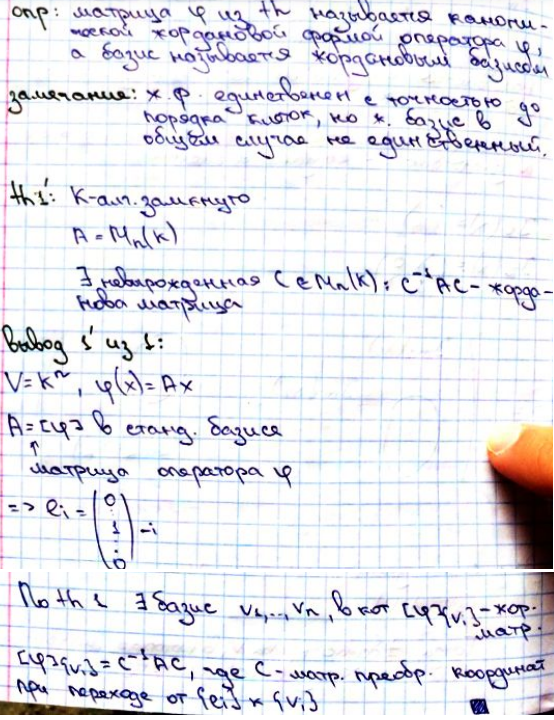
\includegraphics[width=10cm]{pics/58}
              \centering
      \end{figure}

    \section{Относительная линейная независимость. Относительные базисы. Корневые пространства. Лемма о спуске для корневых подпространств.}

    *здесь когда-нибудь будет что-то*

    \begin{lemma}[1]
      *здесь когда-нибудь будет лемма*
    \end{lemma}

    *здесь когда-нибудь будет вывод*

    *здесь когда-нибудь будет что-то*
    \begin{figure}[H]
            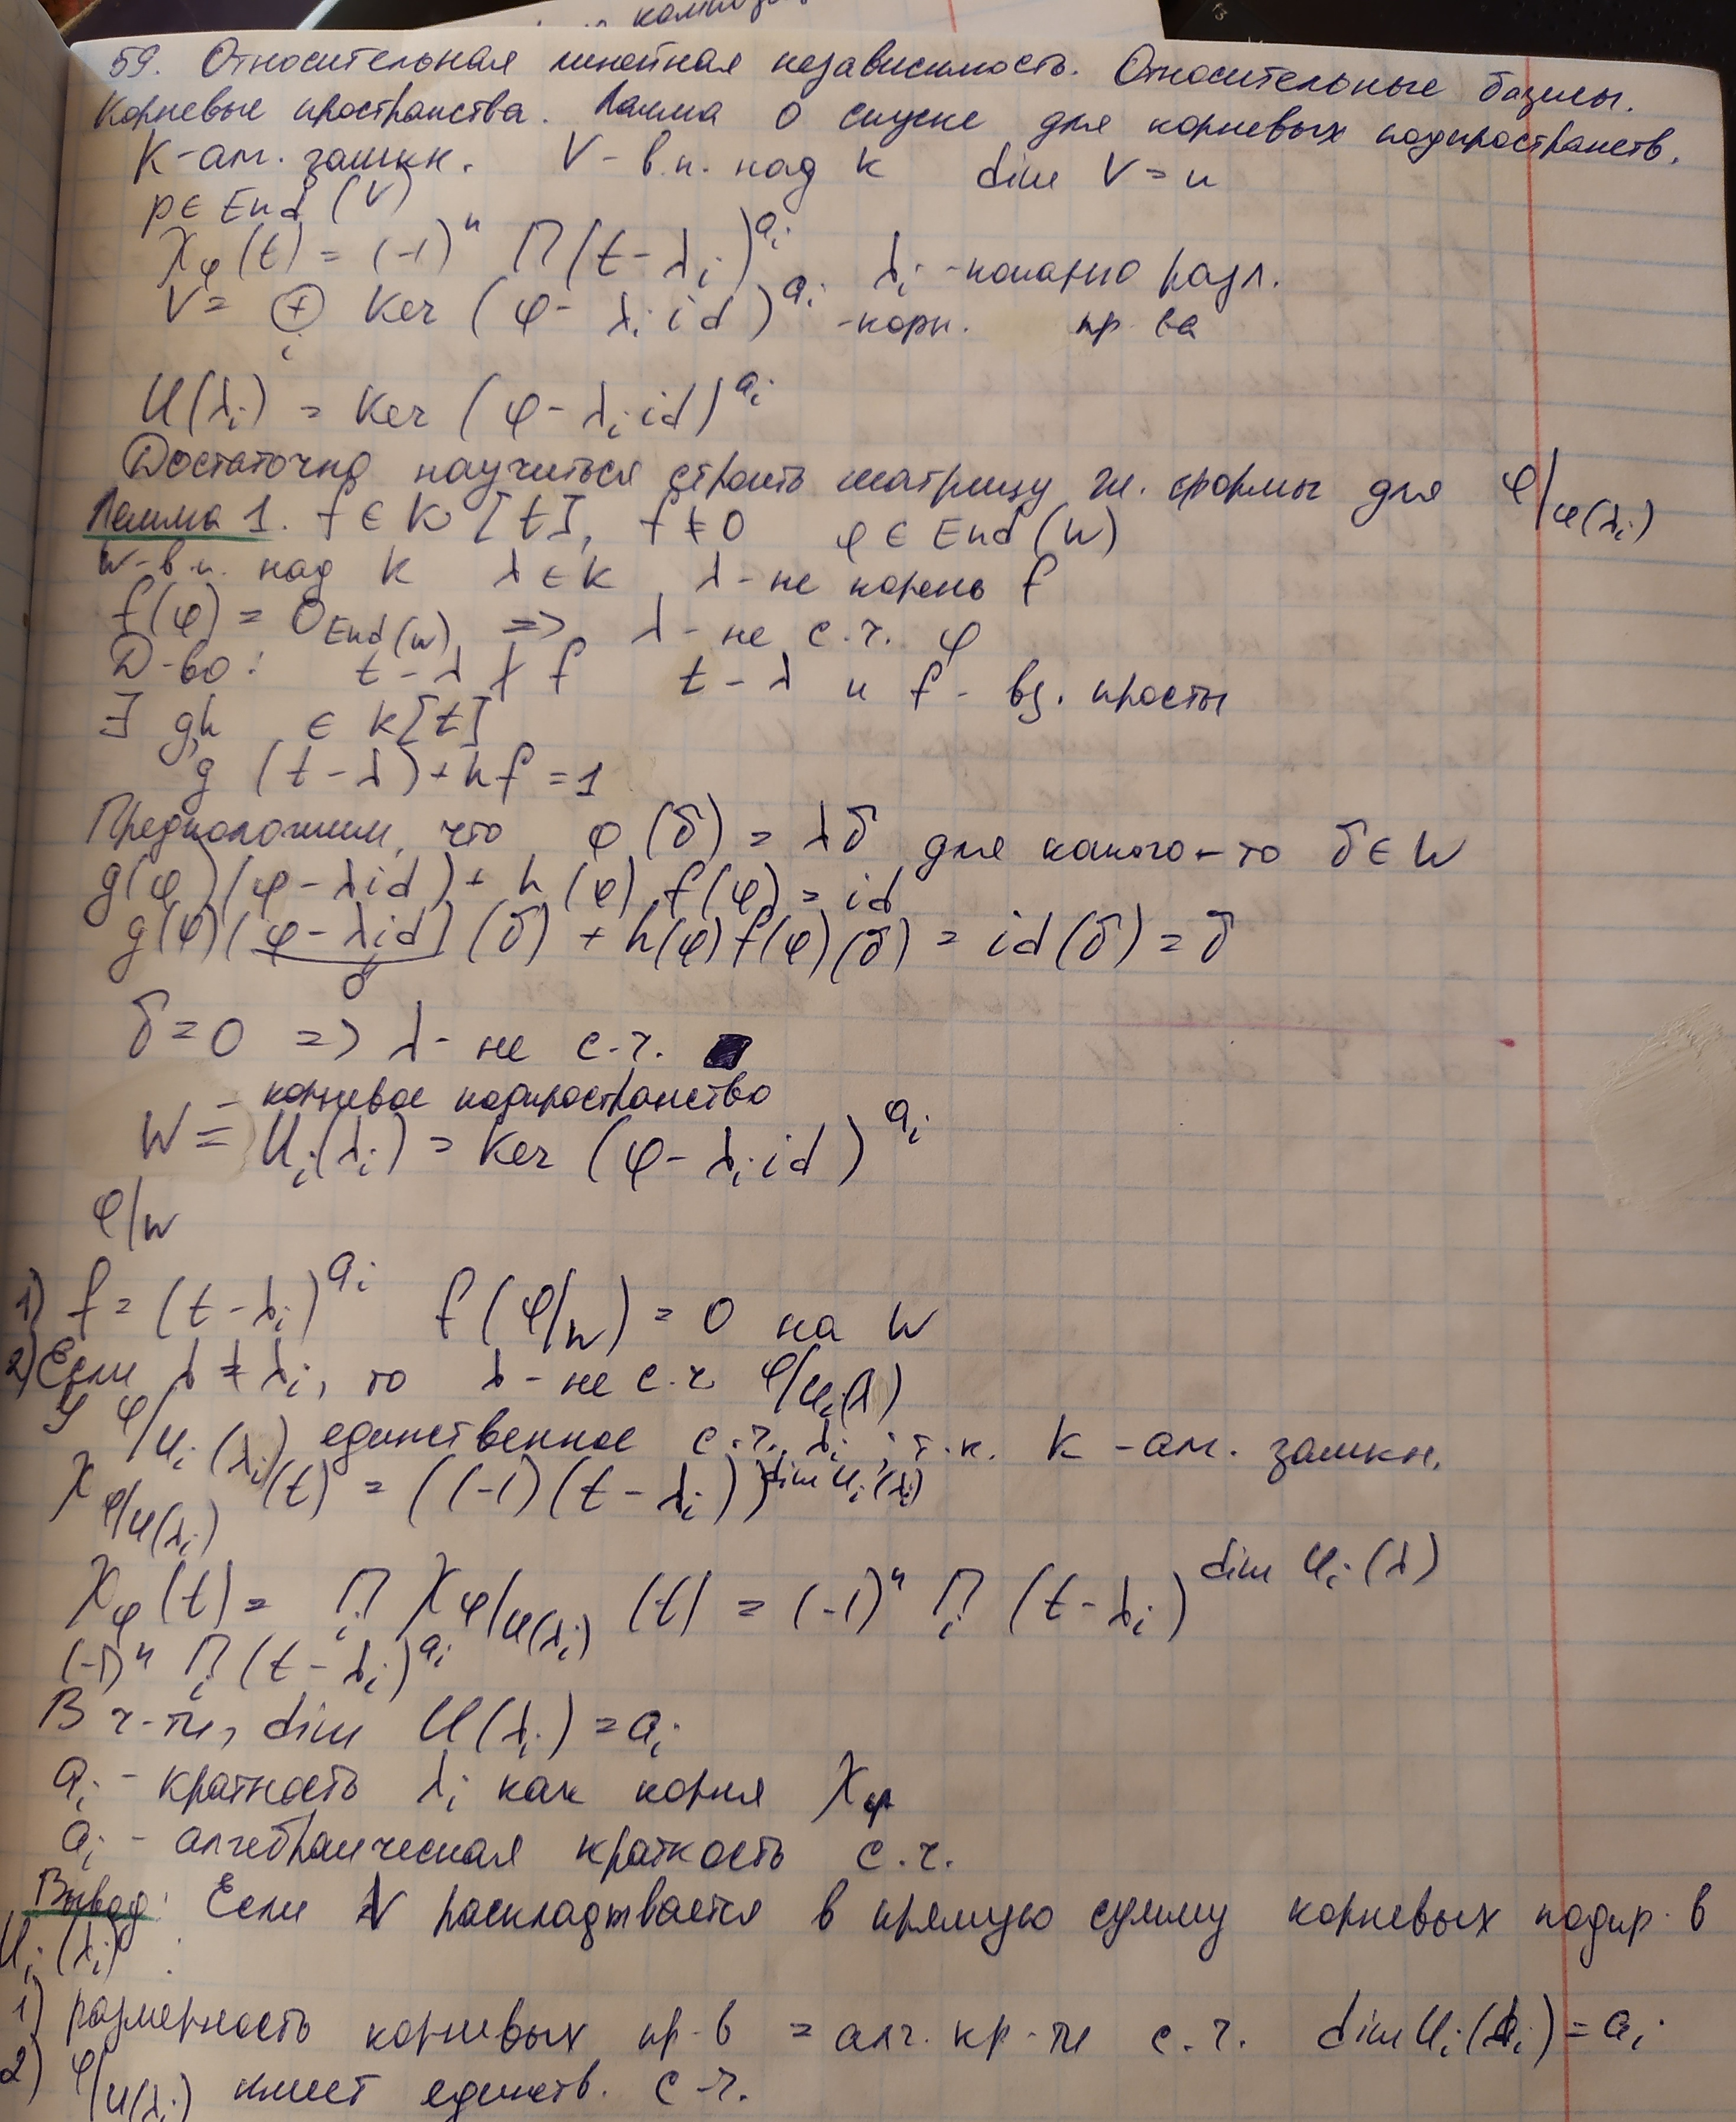
\includegraphics[width=10cm]{pics/l59_1}
            \centering
    \end{figure}
    \begin{figure}[H]
            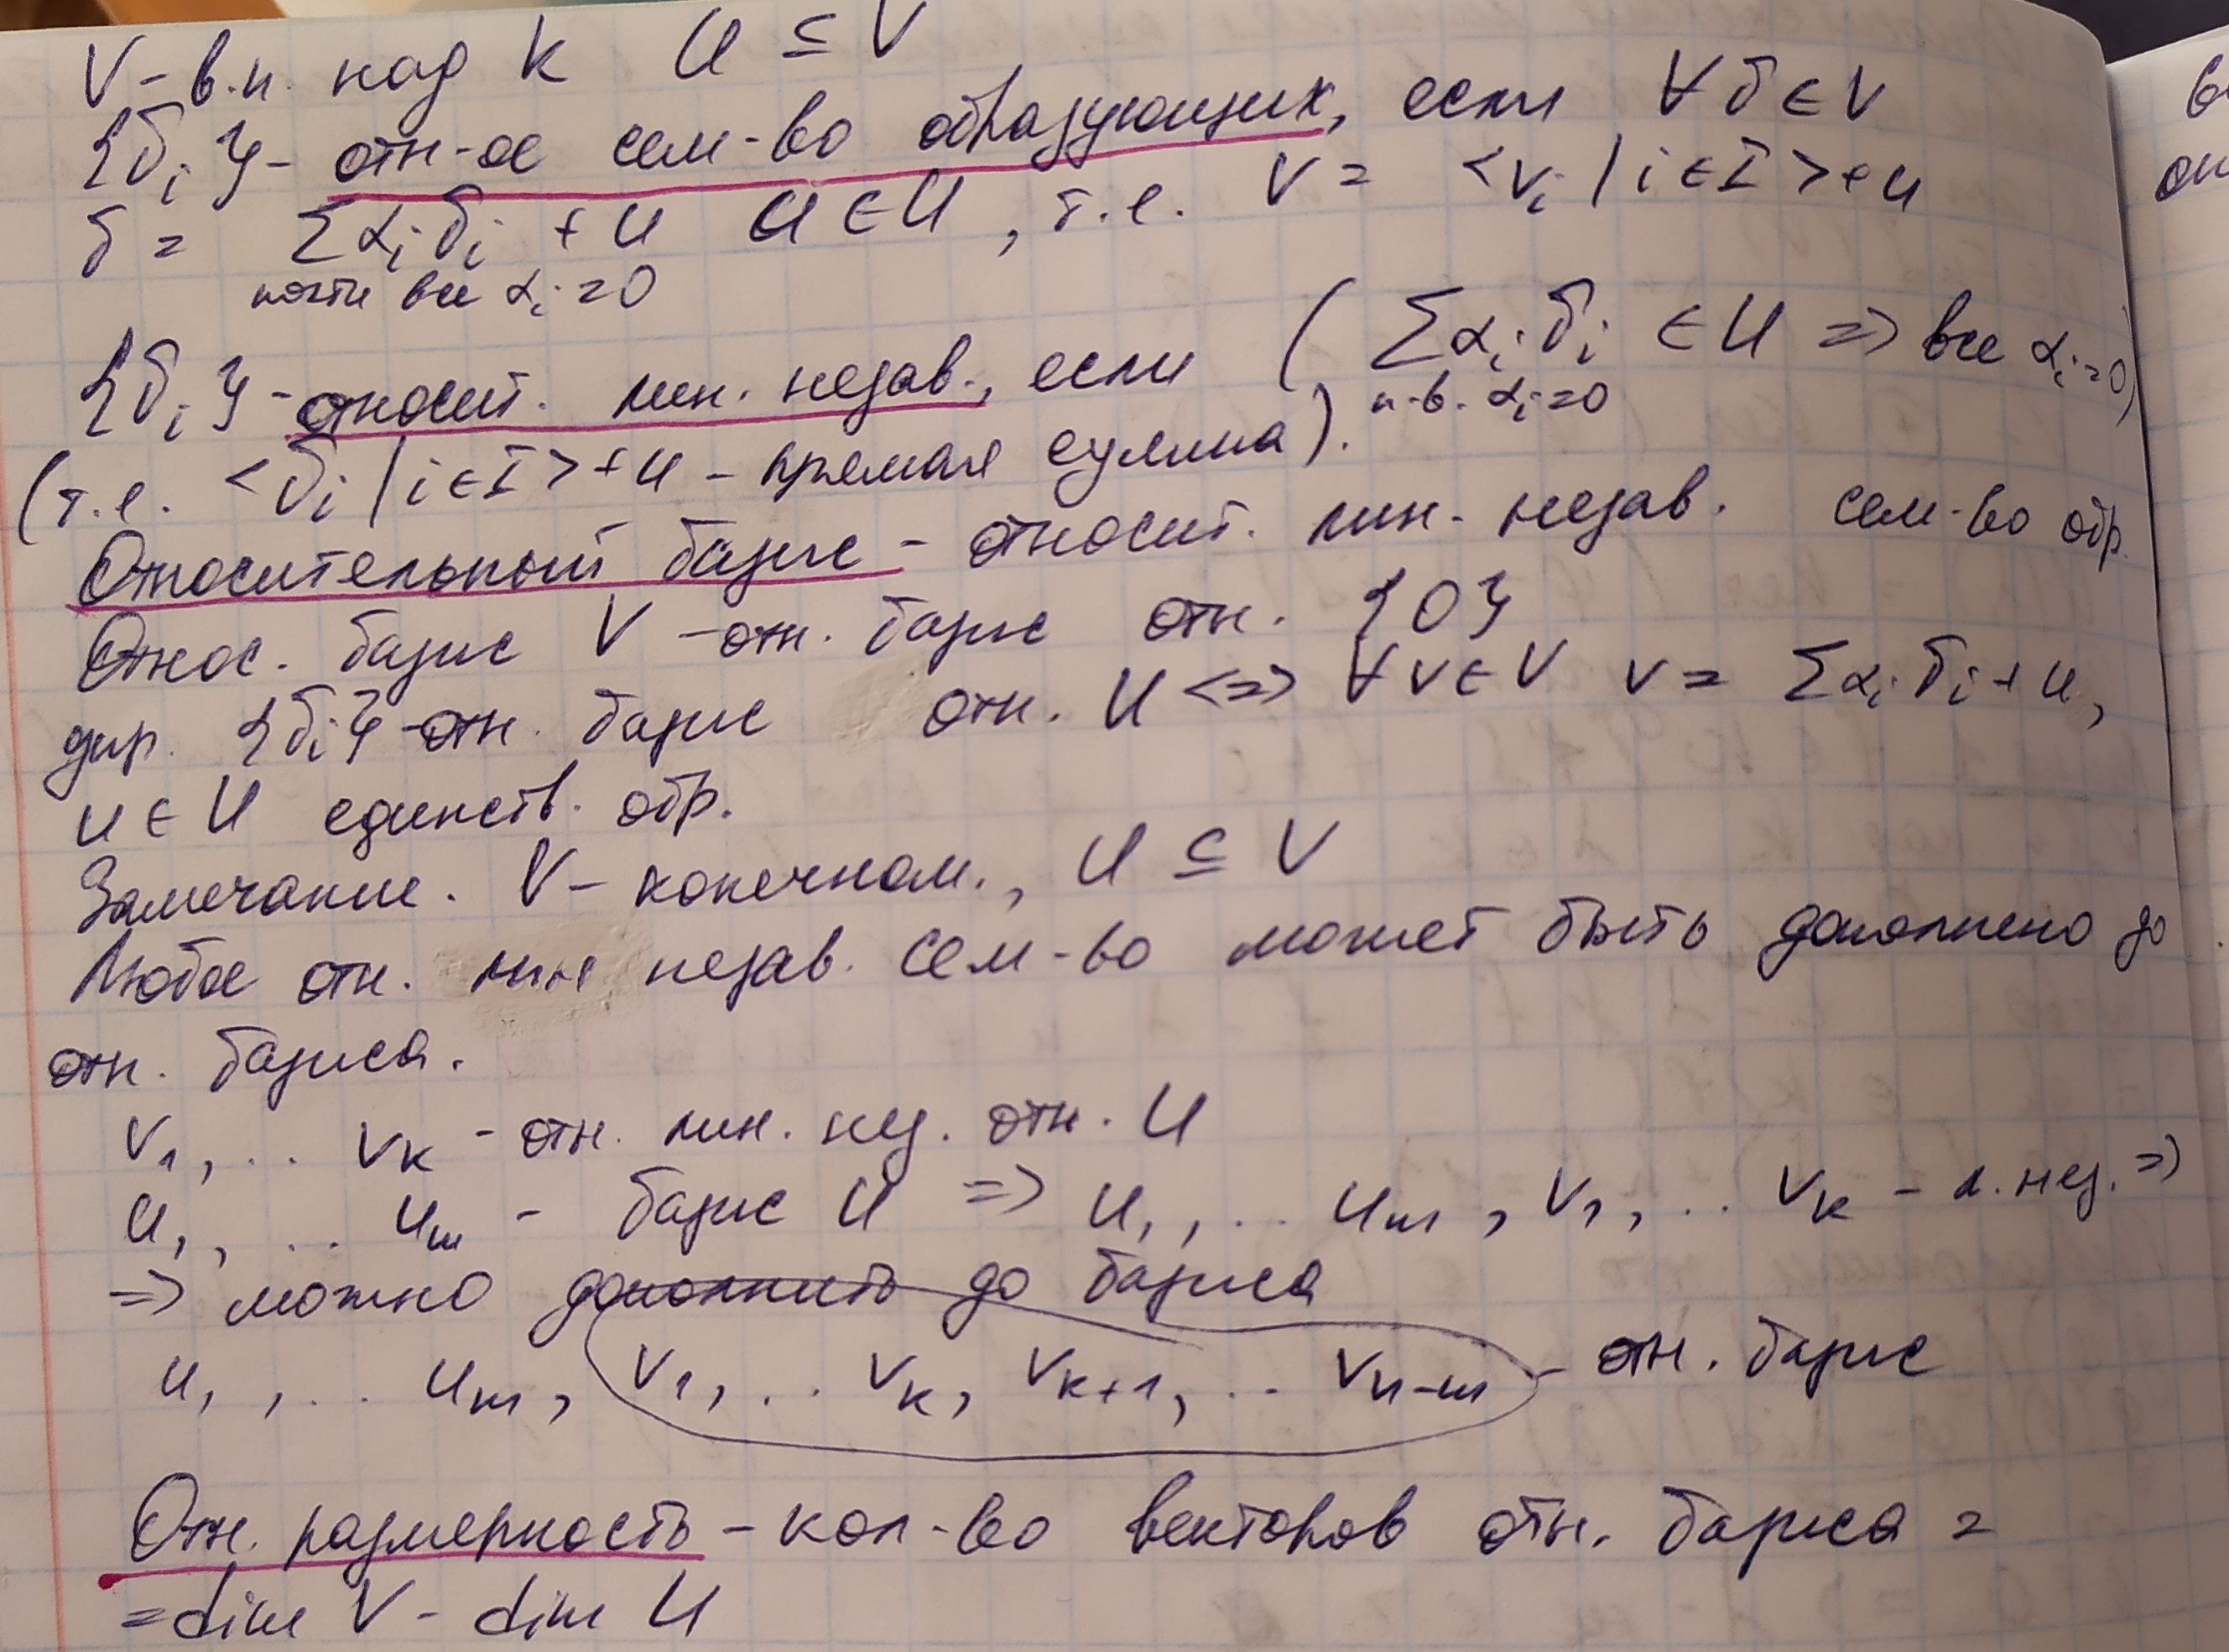
\includegraphics[width=10cm]{pics/l59_2}
            \centering
    \end{figure}

    \section{Построение жорданова базиса и жордановой формы для оператора с единственным собственным числом.}

    *здесь когда-нибудь будет что-то*

    \begin{lemma}[1]
      *здесь когда-нибудь будет лемма*
    \end{lemma}

    \begin{proof}
      *здесь когда-нибудь будет док-во*
    \end{proof}

    \begin{figure}[H]
            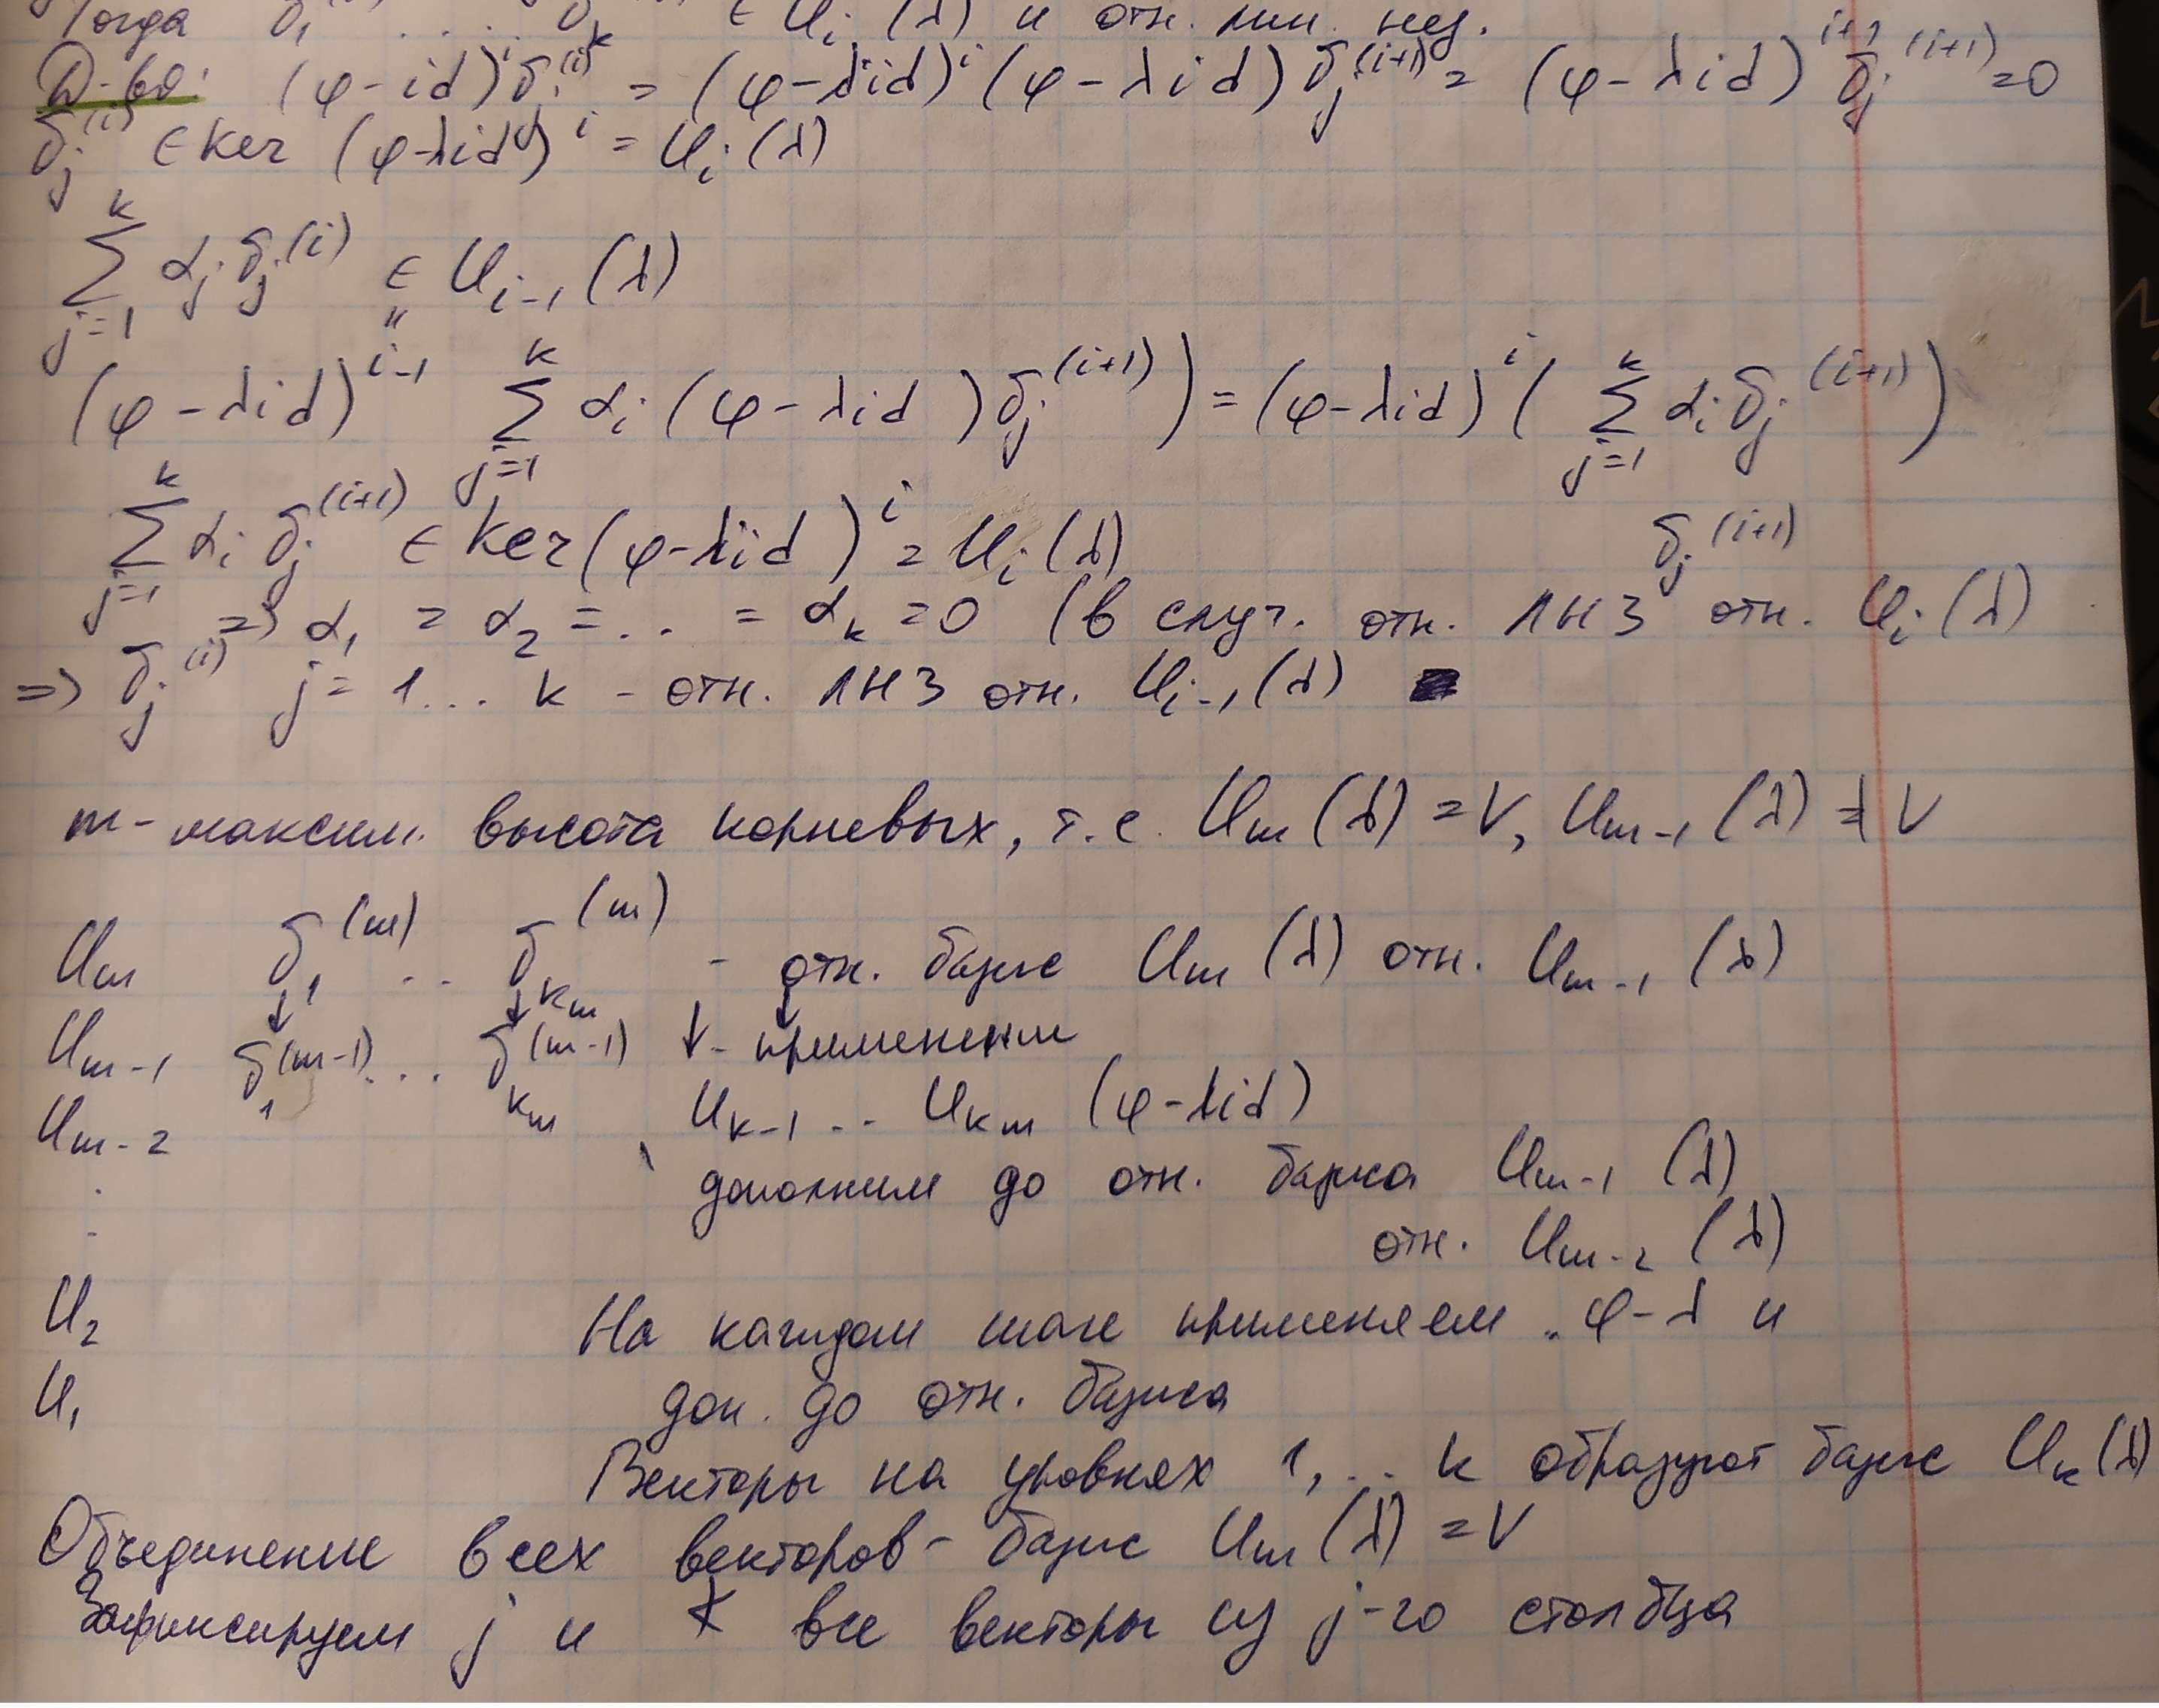
\includegraphics[width=10cm]{pics/l60_1}
            \centering
    \end{figure}

    \begin{figure}[H]
            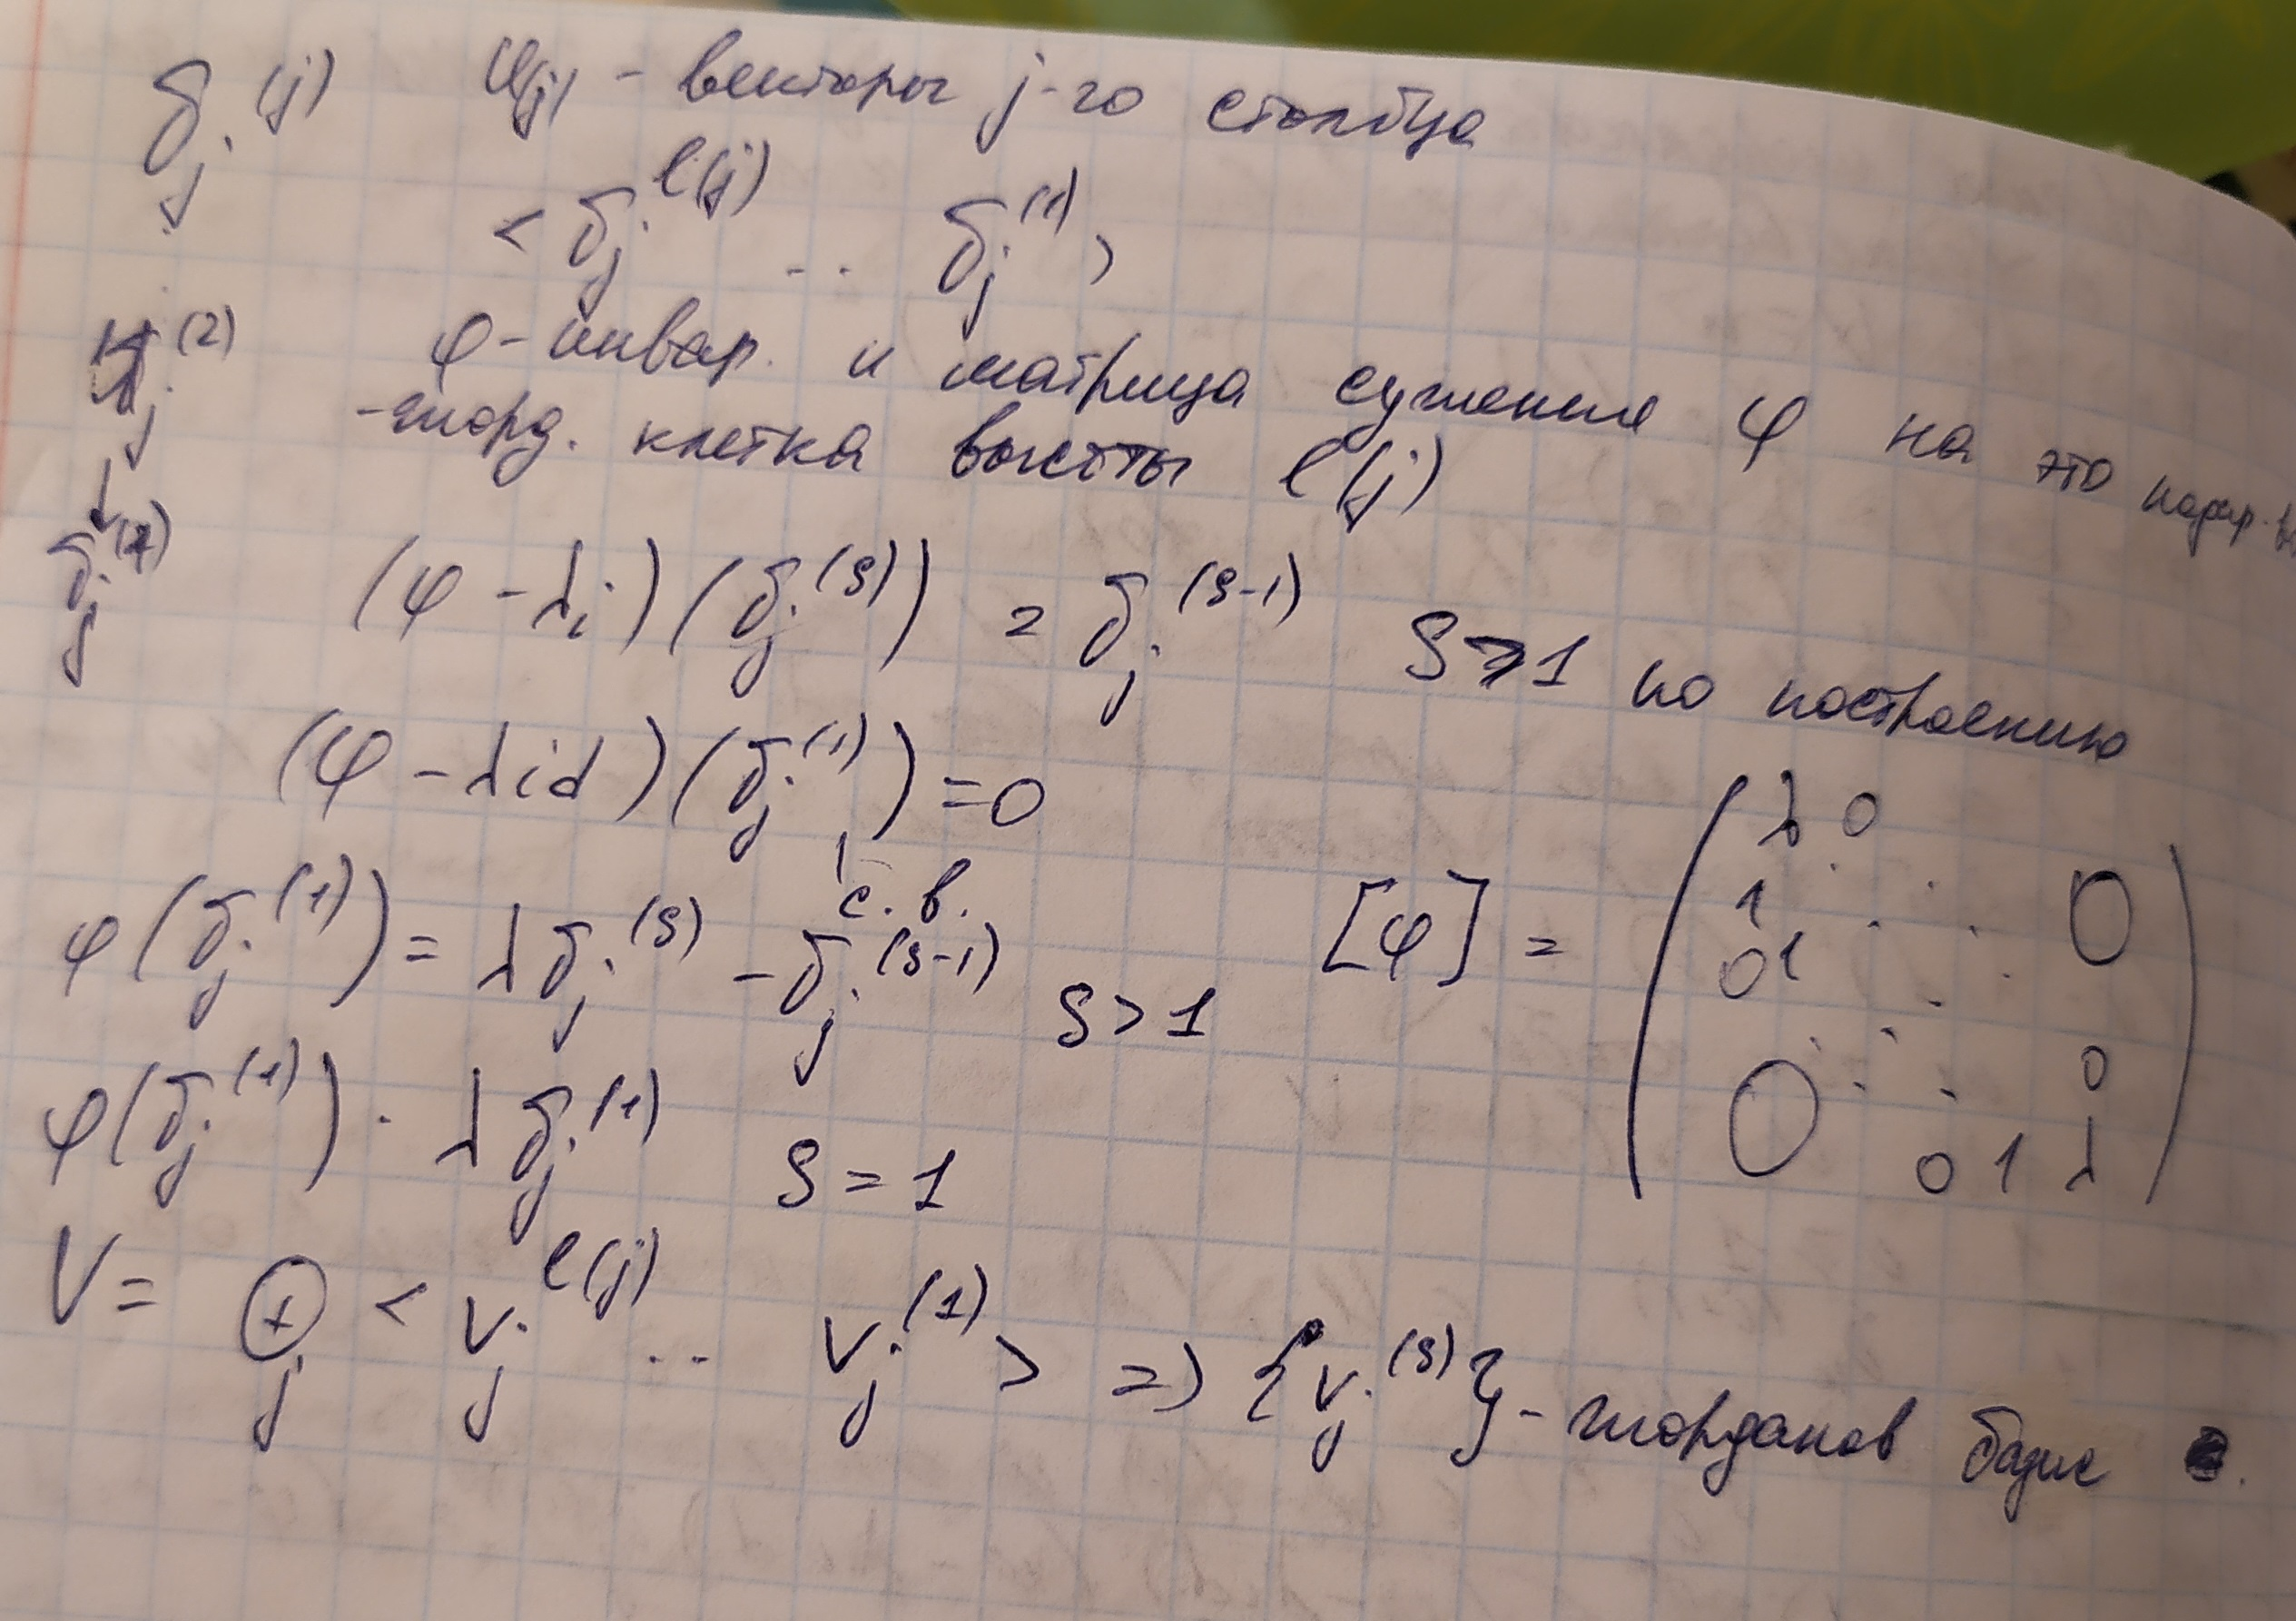
\includegraphics[width=10cm]{pics/l60_2}
            \centering
    \end{figure}

    \section{Единственность жордановой формы оператора.}

    *здесь когда-нибудь будет что-то*

    \begin{consequence}
      *здесь когда-нибудь будет следствие*
    \end{consequence}

    \begin{consequence}
      *здесь когда-нибудь будет следствие*
    \end{consequence}

    \begin{figure}[H]
            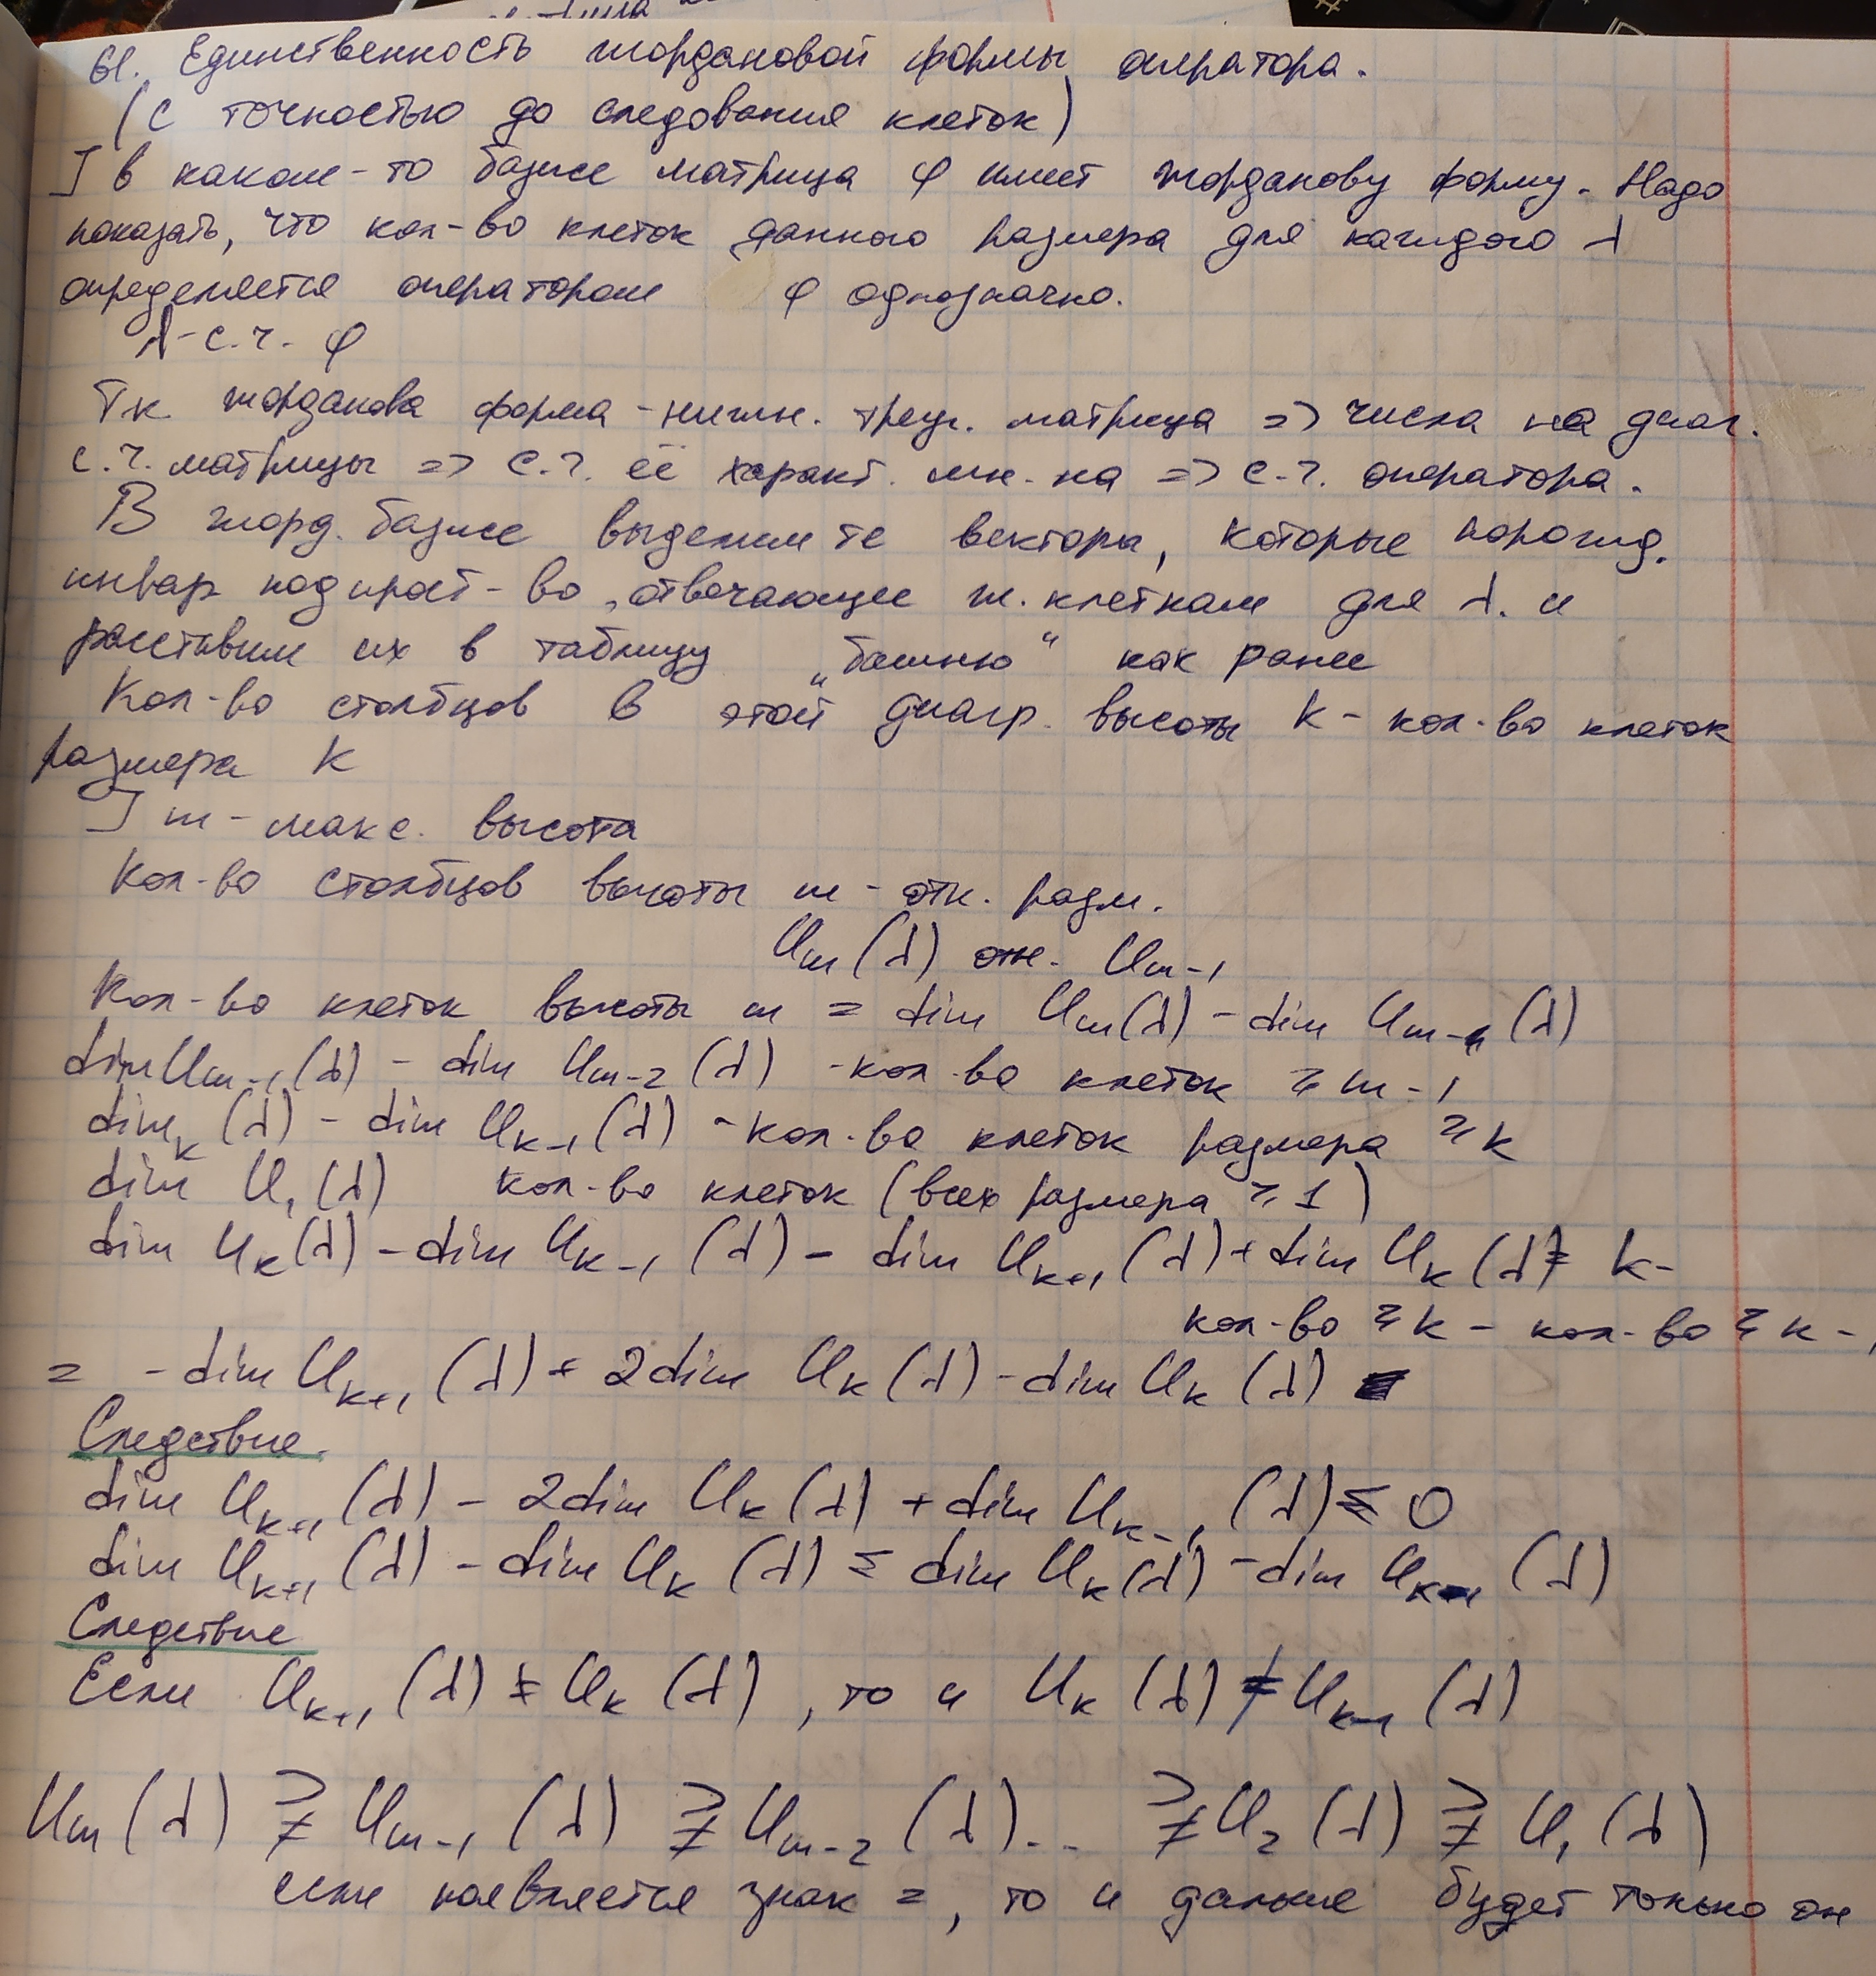
\includegraphics[width=10cm]{pics/l61}
            \centering
    \end{figure}
\end{document}
